%%%%%%%%%%%%%%%%%%%%%%%%%%%%%%%%%%%%%%%%%
% Dreuw & Deselaer's Poster
% LaTeX Template
% Version 1.0 (11/04/13)
%
% Created by:
% Philippe Dreuw and Thomas Deselaers
% http://www-i6.informatik.rwth-aachen.de/~dreuw/latexbeamerposter.php
%
% This template has been downloaded from:
% http://www.LaTeXTemplates.com
%
% License:
% CC BY-NC-SA 3.0 (http://creativecommons.org/licenses/by-nc-sa/3.0/)
%
%%%%%%%%%%%%%%%%%%%%%%%%%%%%%%%%%%%%%%%%%

%----------------------------------------------------------------------------------------
%	PACKAGES AND OTHER DOCUMENT CONFIGURATIONS
%----------------------------------------------------------------------------------------

\documentclass[final]{beamer}

\usepackage[utf8]{inputenc}

\usepackage[orientation=portrait,size=a0,scale=1.4]{beamerposter} % Use the beamerposter package for laying out the poster with a portrait orientation and an a0 paper size

\usetheme{I6pd2} % Use the I6pd2 theme supplied with this template

\usepackage[english]{babel} % English language/hyphenation

\usepackage{amsmath,amsthm,amssymb,latexsym} % For including math equations, theorems, symbols, etc

%\usepackage{times}\usefonttheme{professionalfonts}  % Uncomment to use Times as the main font
%\usefonttheme[onlymath]{serif} % Uncomment to use a Serif font within math environments

%\boldmath % Use bold for everything within the math environment

\usepackage{booktabs} % Top and bottom rules for tables

\usepackage{epstopdf}

\graphicspath{{figures/}} % Location of the graphics files

\usecaptiontemplate{\small\structure{\insertcaptionname~\insertcaptionnumber: }\insertcaption} % A fix for figure numbering

\newcommand{\R}{{\mathbb R}}
\newcommand{\C}{{\mathbb C}}
\newcommand{\N}{{\mathbb N}}
\newcommand{\eps}{\ensuremath{\varepsilon}}

%----------------------------------------------------------------------------------------
%	TITLE SECTION 
%----------------------------------------------------------------------------------------

\title{\LARGE Glottal inversion with an approximate vocal tract filter} % Poster title

\author{Lasse Lybeck, Robert Sirviö} % Author(s)

\institute{University of Helsinki, Department of Mathematics and Statistics} % Institution(s)

%----------------------------------------------------------------------------------------
%	FOOTER TEXT
%----------------------------------------------------------------------------------------

\newcommand{\leftfoot}{} % Left footer text

\newcommand{\rightfoot}{lasse.lybeck@helsinki.fi, robert.sirvio@helsinki.fi} % Right footer text

%----------------------------------------------------------------------------------------

\begin{document}

\addtobeamertemplate{block end}{}{\vspace*{2ex}} % White space under blocks

\begin{frame}[t] % The whole poster is enclosed in one beamer frame

\begin{columns}[t] % The whole poster consists of two major columns, each of which can be subdivided further with another \begin{columns} block - the [t] argument aligns each column's content to the top

\begin{column}{.02\textwidth}\end{column} % Empty spacer column

\begin{column}{.465\textwidth} % The first column


%----------------------------------------------------------------------------------------
%	INTRODUCTION
%----------------------------------------------------------------------------------------
            
\begin{block}{Introduction}

\begin{itemize}
\item A synthetic human vowel sound consists of a periodic signal to simulate the glottal excitation signal at the glottis and a filter to simulate the vocal tract, which the glottal signal is filtered through.\cite{touda} With a given vocal tract filter the direct problem is \emph{given a glottal excitation signal, create the vowel sound}. The inverse problem is \emph{given a (recorded) vowel sound, find the glottal excitation signal}. We will be concentrating on the inverse problem using simulated vowel data.

\item The inversion from a vowel sound to the glottal signal is an important part of creating synthetic human voices and speech generators. To create a synthetic vowel both the glottal signal and the vocal tract filter are needed. However, the glottal signal cannot be directly measured, but it can be approximated with inversion of a recorded vowel. This data can be used to create models for simulating the glottal excitation signal.
\end{itemize}

\end{block}

%----------------------------------------------------------------------------------------
%	MATERIALS AND METHODS
%----------------------------------------------------------------------------------------

\begin{block}{Materials and methods}

\begin{columns} % Subdivide the first main column
\begin{column}{.6\textwidth} % The first subdivided column within the first main column

\begin{itemize}

\item The \emph{Rosenberg-Klatt model} (\emph{RK-model)} \cite{rosenberg} was used to simulate the \emph{glottal excitation signal}. The parameters used by the model are the sound frequency $f$ and the \emph{klatt-parameter} $Q$. An example of the resulting airflow and pressure can be seen in figure \ref{fig:klatt}.

\end{itemize}

\end{column}

\begin{column}{.38\textwidth} % The second subdivided column within the first main column

\begin{figure}[t]
\begin{center}
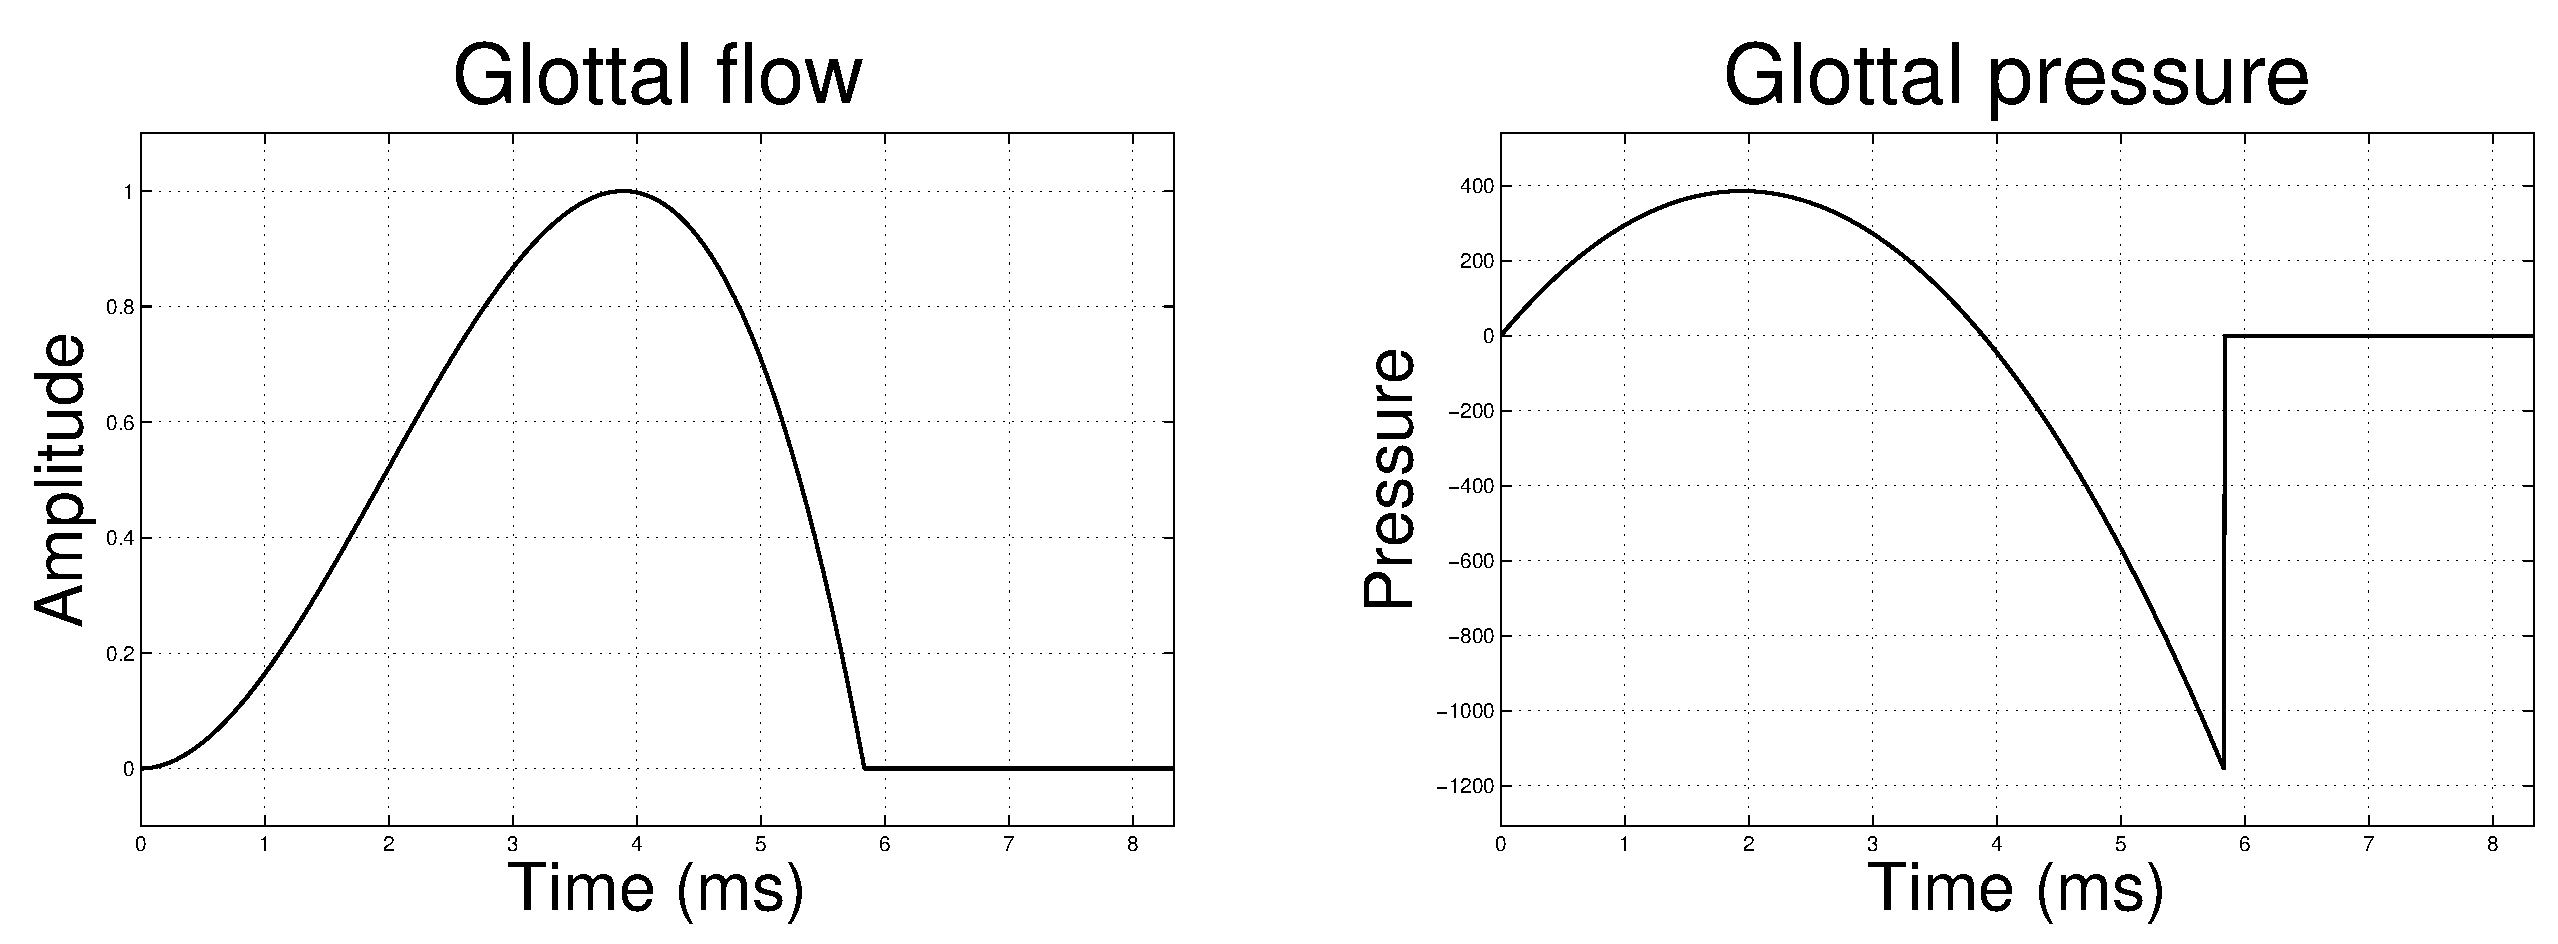
\includegraphics[width=\linewidth]{klatt.eps}
\end{center}
\caption{The airflow and pressure generated by the RK-model}
\label{fig:klatt}
\end{figure}

\end{column}
\end{columns} % End of the subdivision

\begin{itemize}

\item The measurement data for the inversion was created synthetically using the RK-model and a digital filter for a (female) vowel /a/. Some random errors were added to the data to simulate measurement noise.

\item The vocal tract filter used in the inversion is a digital filter simulating the (male) vowel /a/. A matrix corresponding to the filter was constructed to arrive at a matrix model $m = A g + \eps$ for the vowel simulation.

\item Even though the filter used in the inversion is not the same as the one used in simulating the data, they were assumed to simulate roughly the same sound when applied on the glottal impulse (the vowel /a/). Therefore the inversion could be done without the fear of inverse crime, while still expecting good results.

\item The inverse problem was solved using the \emph{Tikhonov regularization} with a customized penalty matrix. The regularization parameter was chosen using \emph{Morozov's discrepancy principle}.

\end{itemize}

\end{block}



%----------------------------------------------------------------------------------------
%	RESULTS
%----------------------------------------------------------------------------------------

\begin{block}{Results}

\begin{itemize}

\item Figure \ref{fig:naive} shows a naïve reconstruction attempt of the glottal excitation signal. In figure \ref{fig:naive-tik} the same inverse problem is solved with Tikhonov regularization using the regularization parameter $\alpha = 75.4$ attained with Morozov's discrepancy principle. The relative error for the naïve reconstruction was $\delta_{\text{rel}} \approx 238 \%$, and for the regularized solution $\delta_{\text{rel}} \approx 66.3 \%$. The measurement data was created with the parameter values $f = 120 \text{Hz}$ and $Q = 0.6$.

\item The relative error of the reconstruction with different values of the regularization parameter $\alpha$ is shown in figure \ref{fig:alpha-iter}. The least error $\delta_{\text{rel}} \approx 64.6 \%$ was attained with the value $\alpha = 201$. Figure \ref{fig:iter-tik} shows the reconstruction of the same data done with Tikhonov regularization. The value of the regularization parameter $\alpha = 104.5$ was chosen with Morozov's discrepancy principle, and resulted in a relative error $\delta_{\text{rel}} \approx 65.0 \%$. The measurement data was created with the parameter values $f = 120 \text{Hz}$ and $Q = 0.5$.

\item The relative error is calculated with the formula
\begin{equation*}
\delta_{rel} = \frac{\left\| g - T_{\alpha}(m) \right\|_2}{\left\| g \right\|_2} \cdot 100 \%,
\end{equation*}
where $g \in \R^k$ is the original glottal excitation signal and $T_{\alpha}(m)$ is the reconstruction calculated from the noisy data $m$ with the regularization parameter $\alpha$.

\item In the figures \ref{fig:naive}, \ref{fig:naive-tik} and \ref{fig:iter-tik} the green line shows the original glottal signal and the blue line shows the reconstruction.

\end{itemize}

\end{block}



%----------------------------------------------------------------------------------------
%	COLUMN BREAK
%----------------------------------------------------------------------------------------

\end{column} % End of the first column

\begin{column}{.03\textwidth}\end{column} % Empty spacer column

%----------------------------------------------------------------------------------------
%	SECOND COLUMN
%----------------------------------------------------------------------------------------

\begin{column}{.465\textwidth} % The second column




%----------------------------------------------------------------------------------------
%	RESULT FIGURES
%----------------------------------------------------------------------------------------

\begin{block}{Results: Figures}


% inverse crime comparison
\begin{columns}

\begin{column}{.5\textwidth}
\begin{center}
\begin{figure}
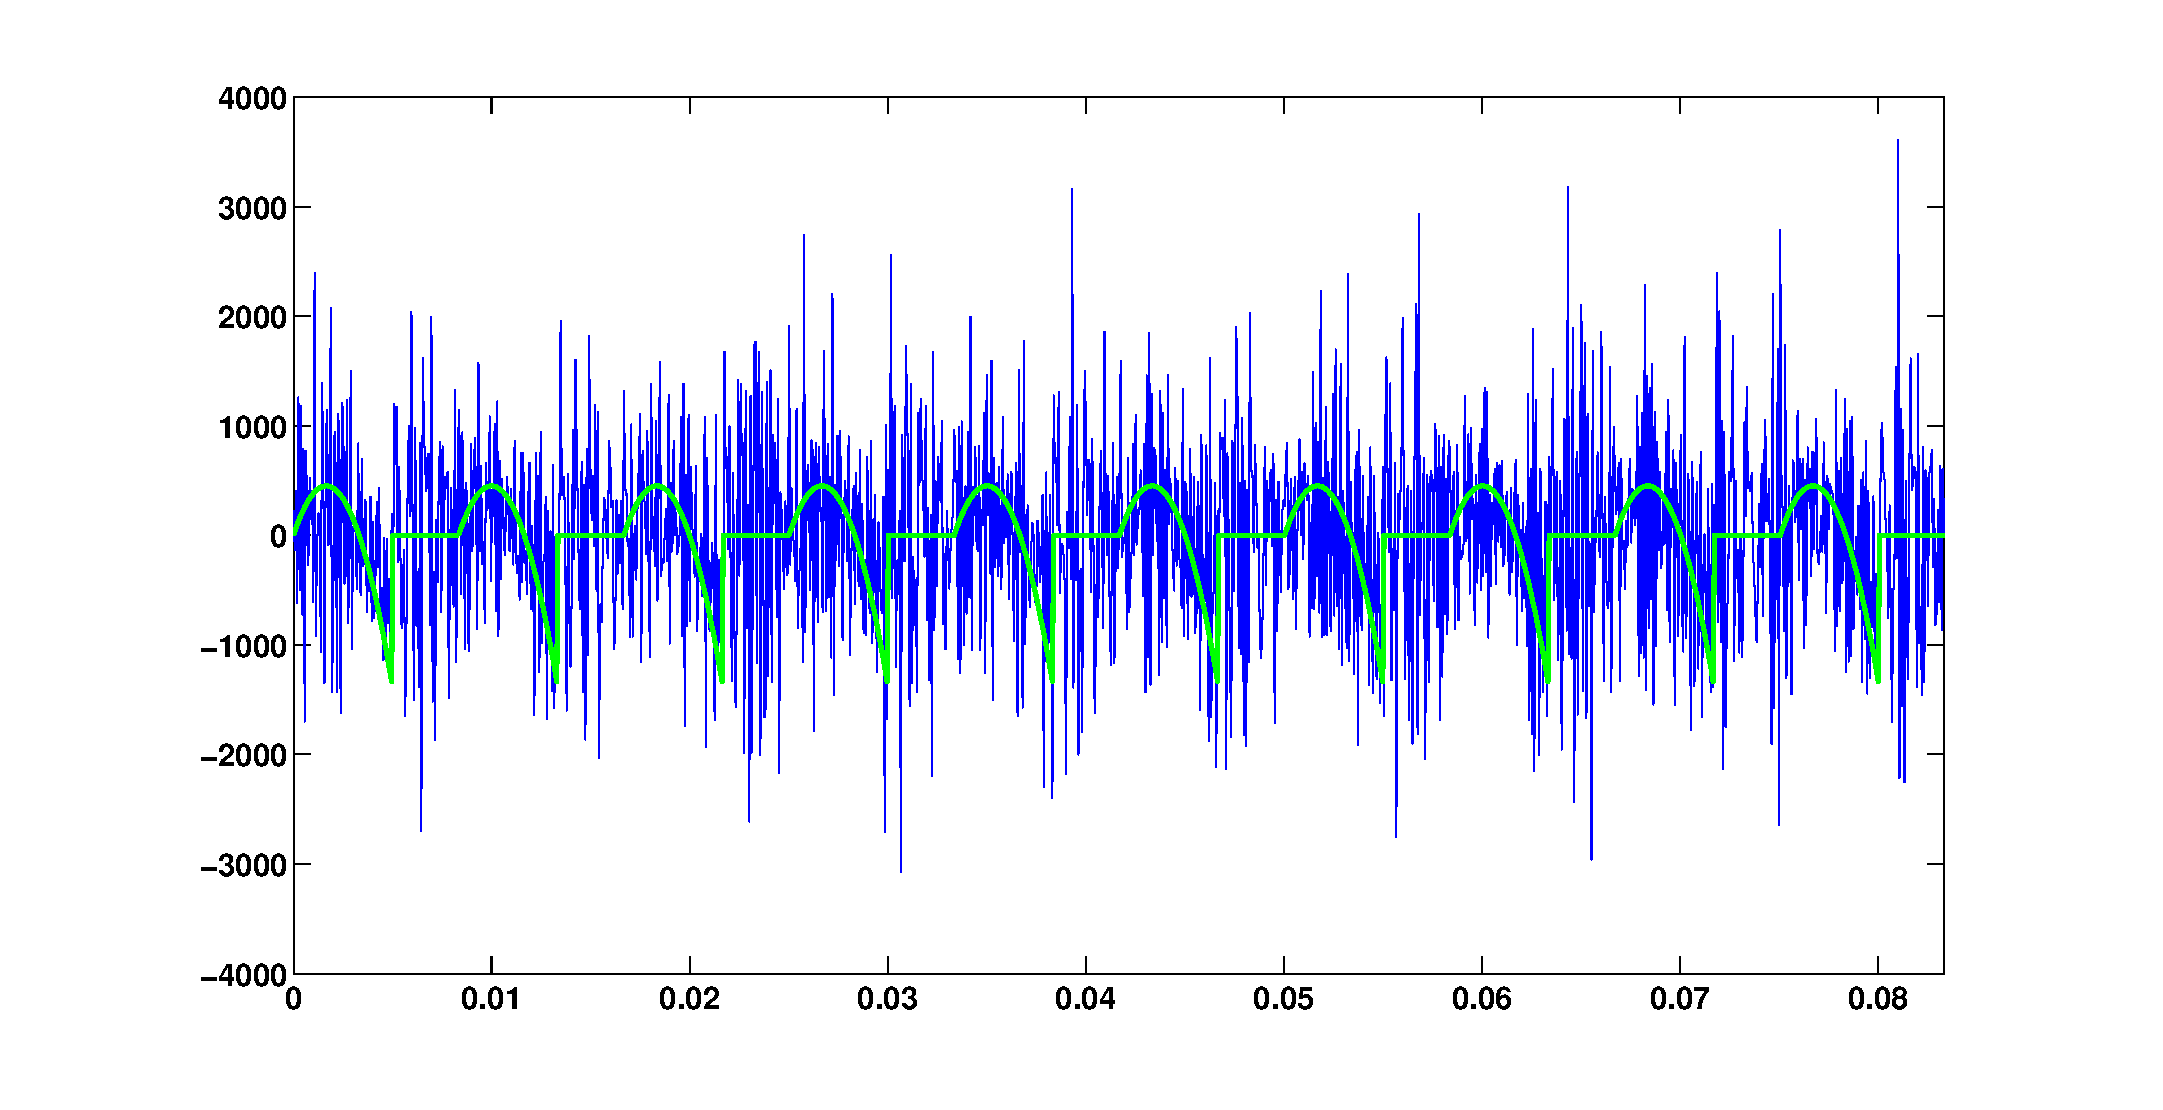
\includegraphics[width=.95\linewidth]{naive_test_nocrime.eps}
\caption{Naïve inversion}
\label{fig:naive}
\end{figure}
\end{center}
\end{column}

\begin{column}{.5\textwidth}
\begin{center}
\begin{figure}
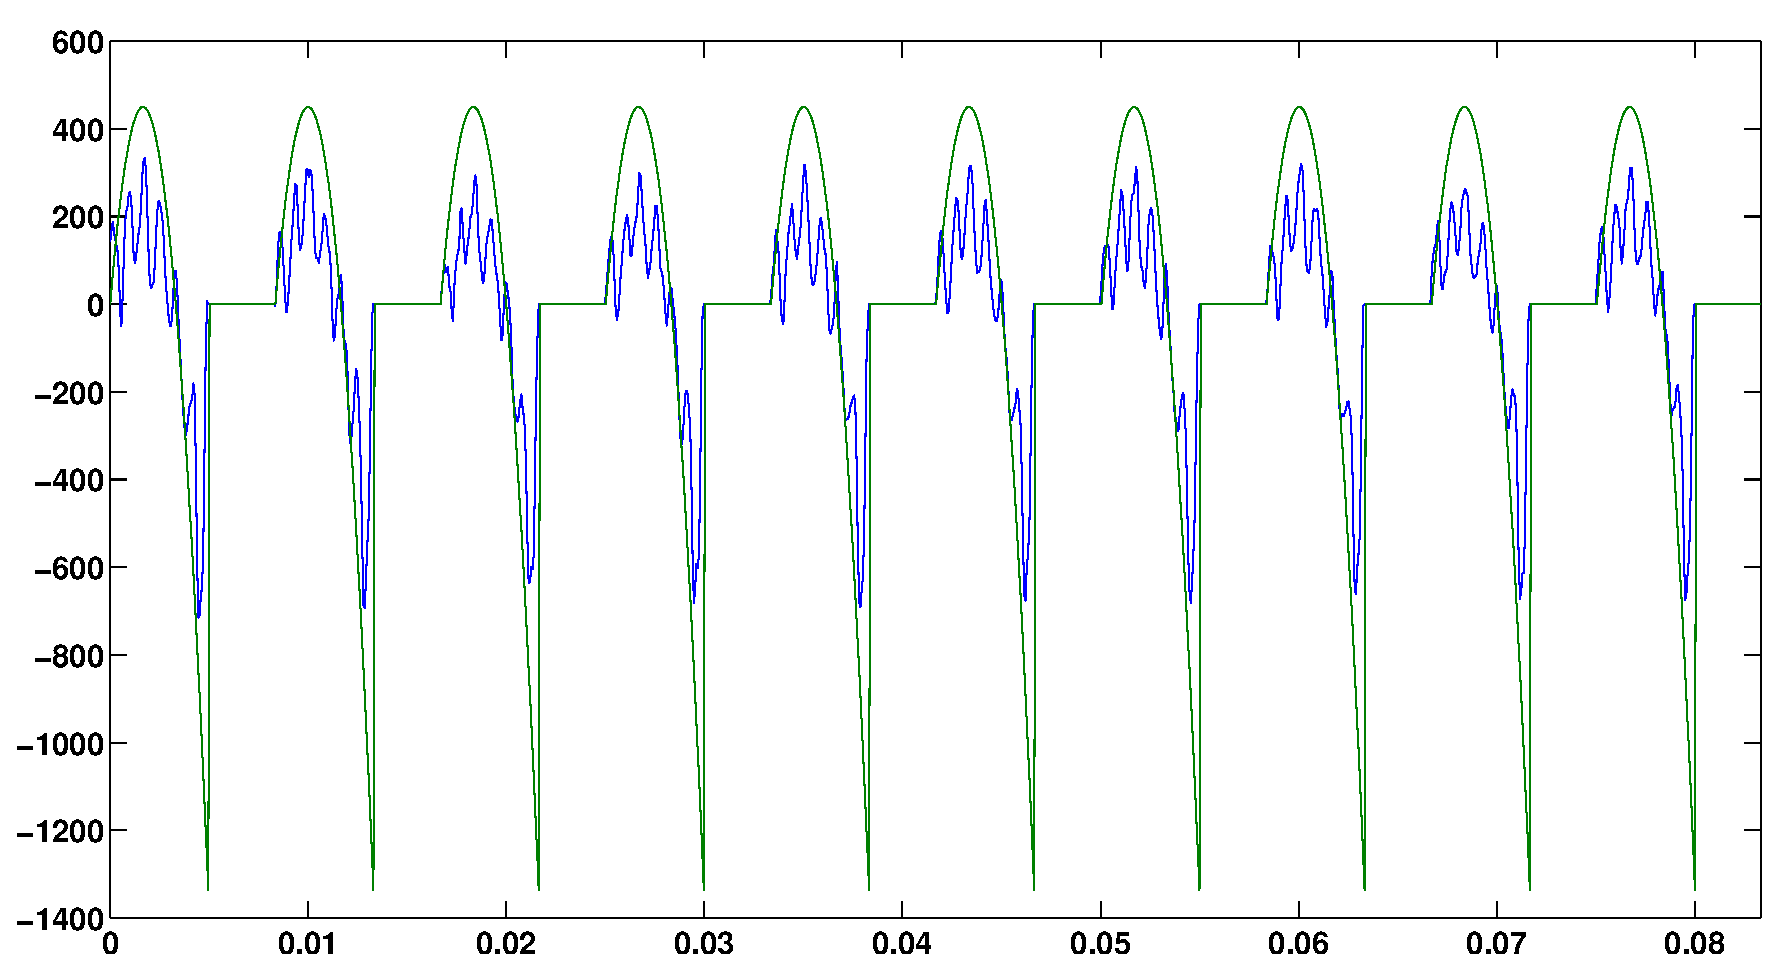
\includegraphics[width=.9\linewidth]{naive_test_nocrime_morozov.eps}
\caption{Tikhonov regularized solution}
\label{fig:naive-tik}
\end{figure}
\end{center}
\end{column}

\end{columns}
% inverse crime comparison END

\vspace{1cm}

% Morozov comparison
\begin{columns}

\begin{column}{.5\textwidth}
\begin{center}
\begin{figure}
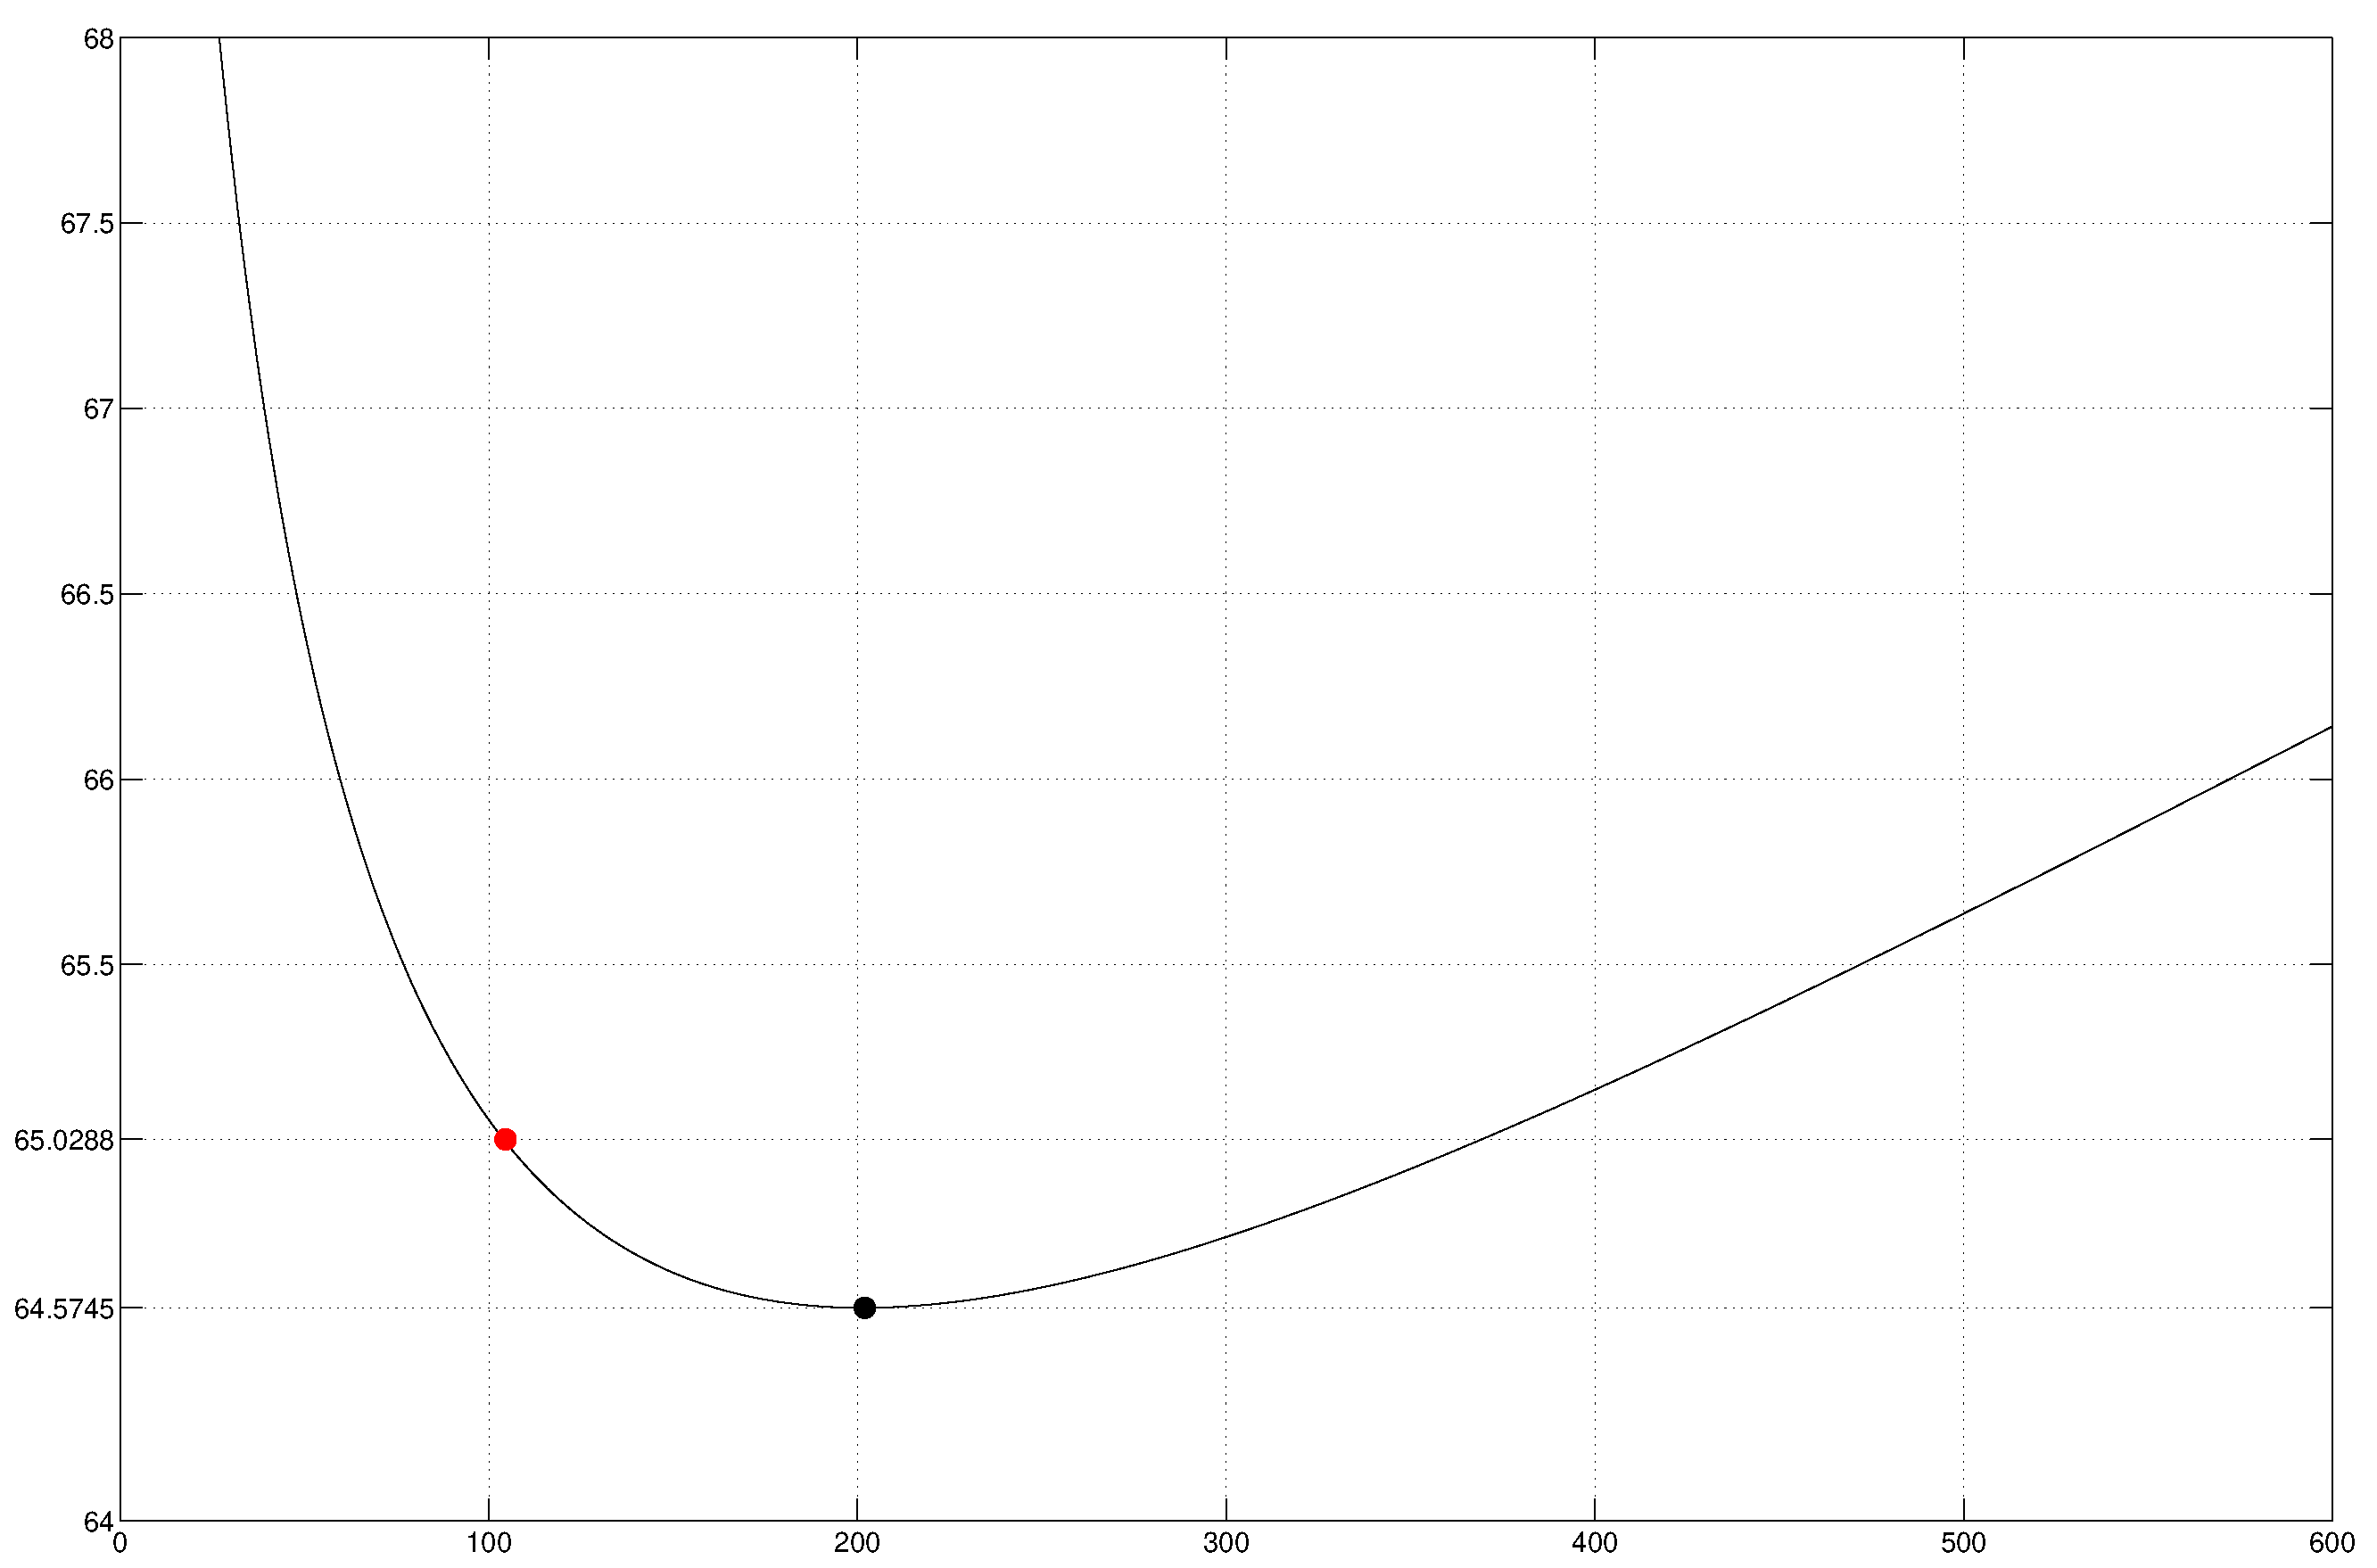
\includegraphics[width=.95\linewidth]{alpha_errs_iter.eps}
\caption{Relative error (\%) by $\alpha$-value}
\label{fig:alpha-iter}
\end{figure}
\end{center}
\end{column}

\begin{column}{.5\textwidth}
\begin{center}
\begin{figure}
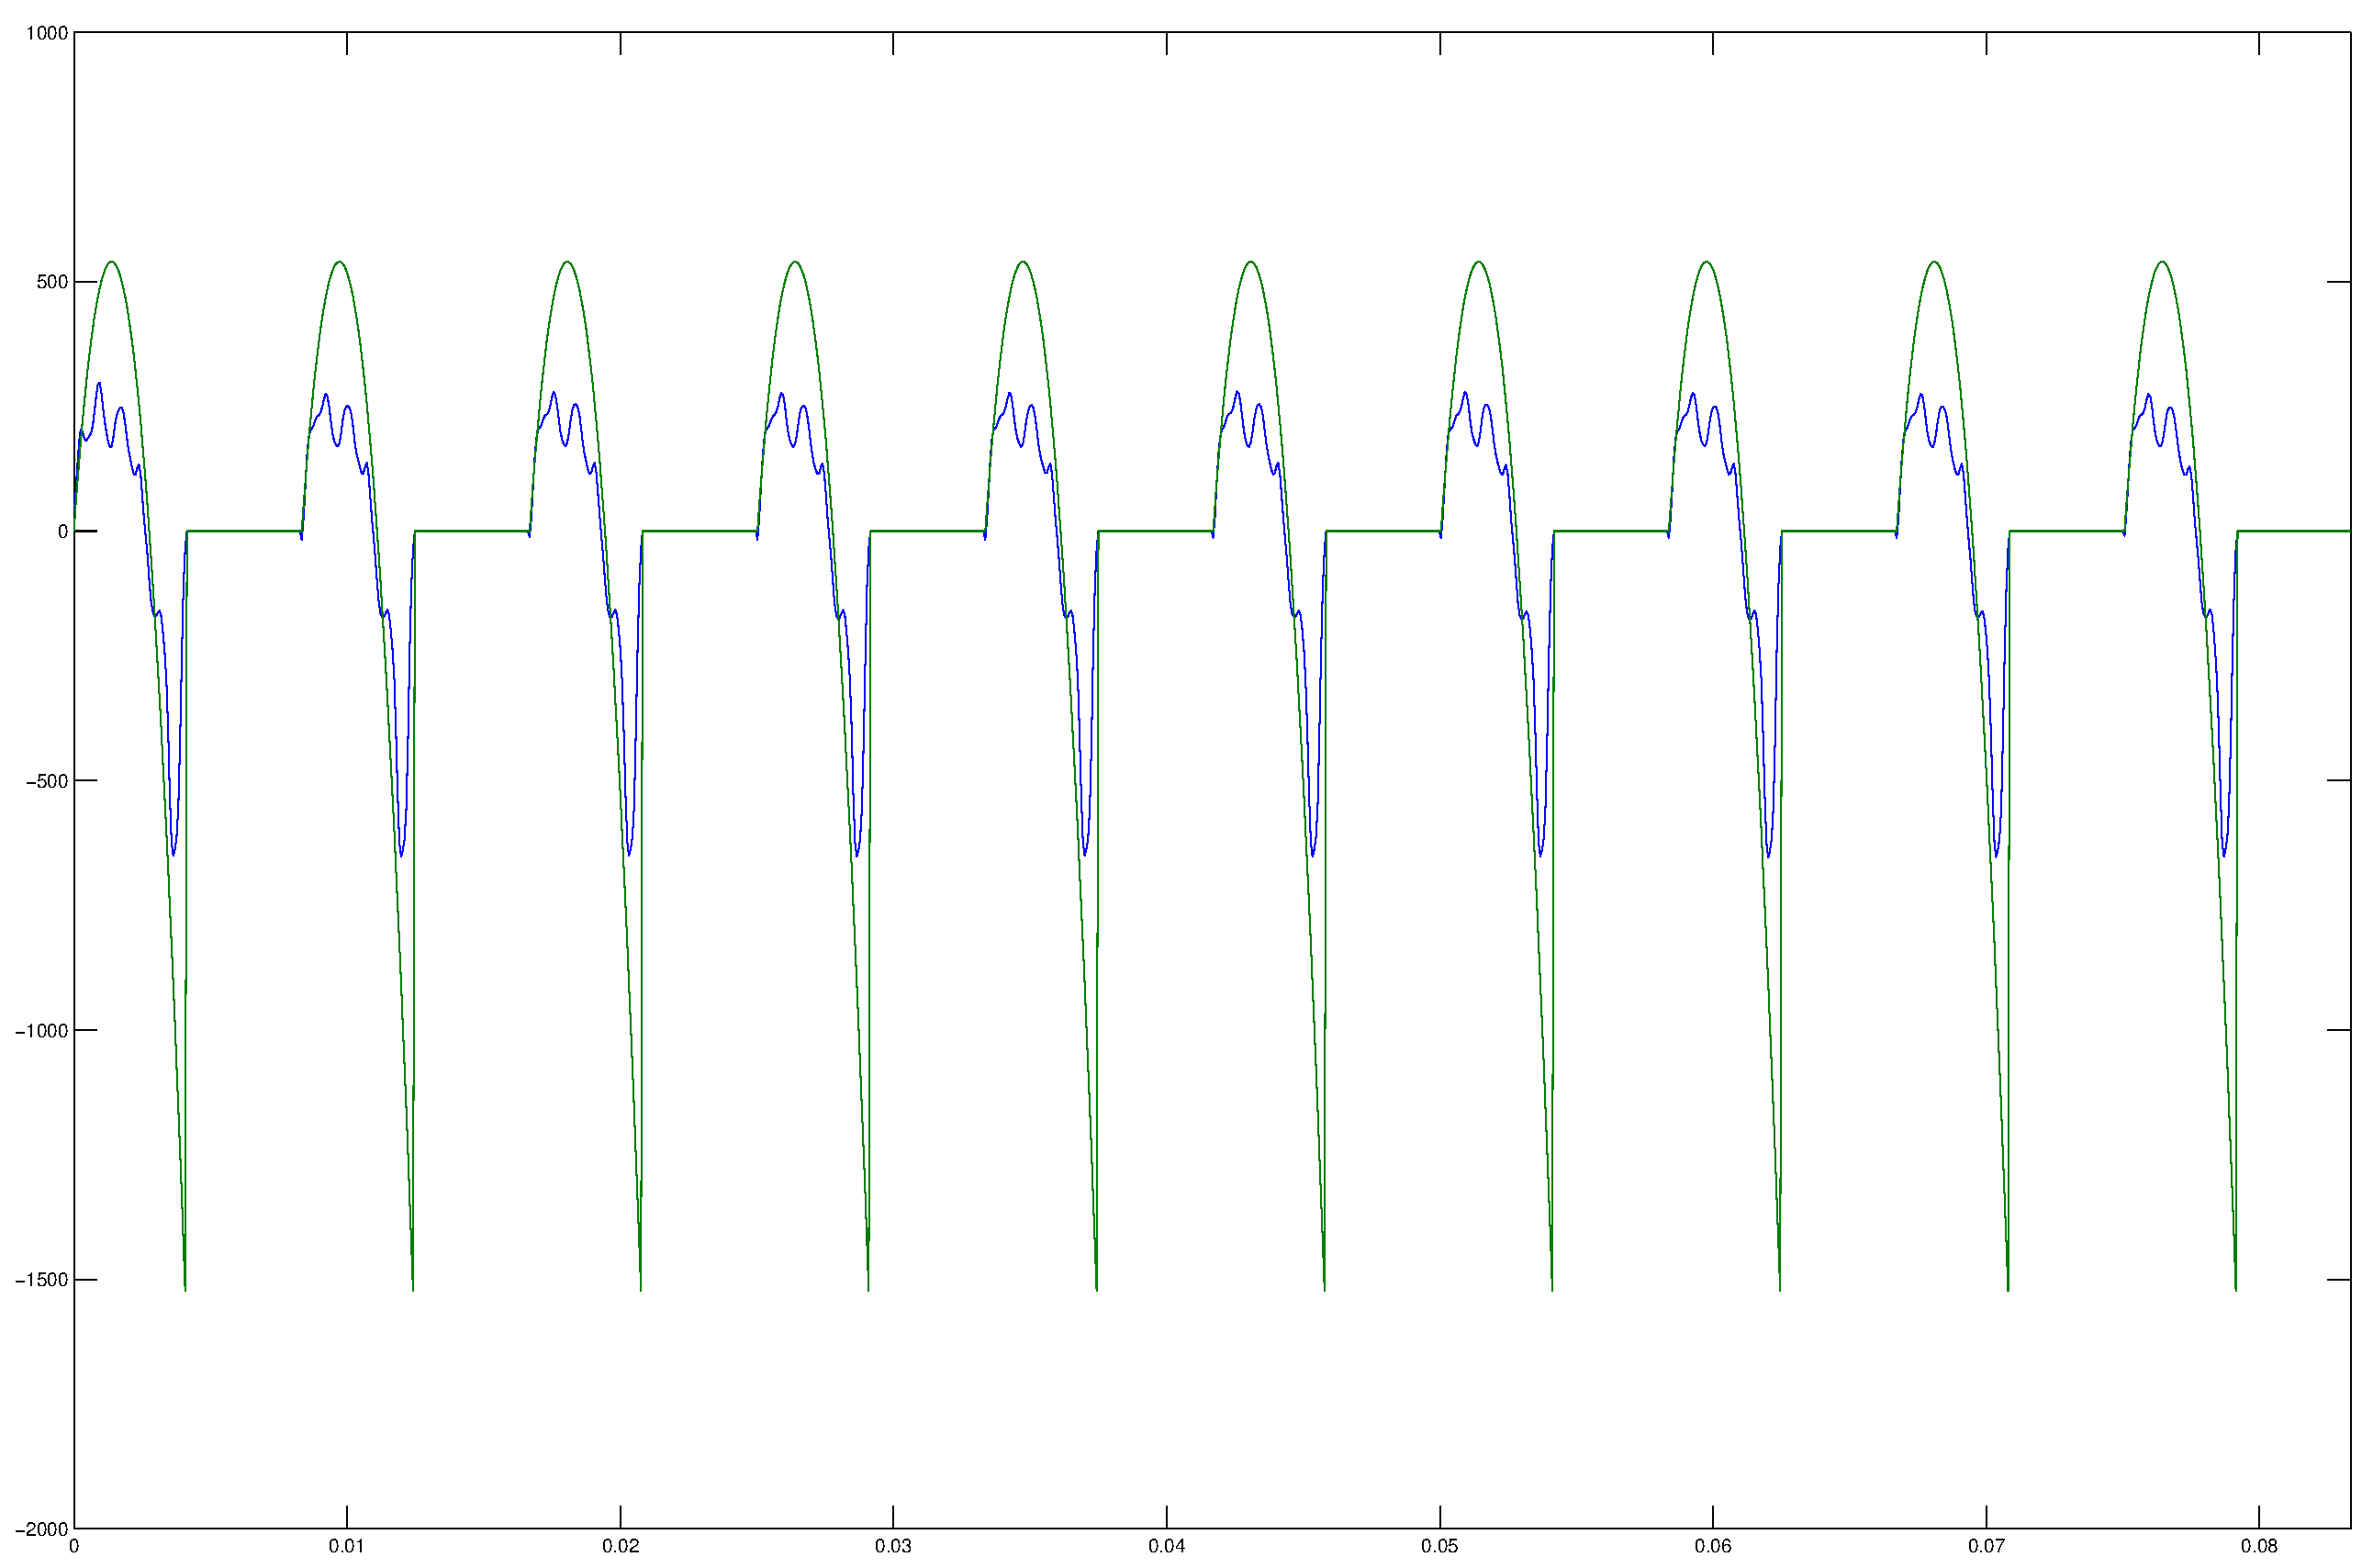
\includegraphics[width=.95\linewidth]{alpha_errs_morozov.eps}
\caption{Tikhonov regularized solution}
\label{fig:iter-tik}
\end{figure}
\end{center}
\end{column}

\end{columns}
% Morozov comparison END


\end{block}

%----------------------------------------------------------------------------------------
%	DISCUSSION
%----------------------------------------------------------------------------------------

\begin{block}{Discussion}



\end{block}

%----------------------------------------------------------------------------------------
%	REFERENCES
%----------------------------------------------------------------------------------------

\begin{block}{References}

\begin{scriptsize}


\begin{thebibliography}{9}

\bibitem{fant}
    Fant, G., Liljencrants, J., Lin, Q., (1985).
    \emph{A four-parameter model of glottal flow}.
    STL-QPSR 26 (4), p. 1-13
    
\bibitem{fujisaki}
    Fujisaki, H., Ljungqvist, M., 1986.
    Proposal and evaluation of models for the glottal source waveform.
    In: Proc. IEEE International Conference on Acoustics, Speech and Signal Processing (ICASSP). Vol. 11. p. 1605–1608.
    
\bibitem{samu}
	Mueller, Jennifer L. \& Siltanen Samuli, (2012).
	\emph{Linear and Nonlinear Inverse Problems with Practical Applications}.
	SIAM, 1:st edition.
	
\bibitem{touda}
    Touda, K., (2007)
    \emph{Study on numerical method for voice generation problem}.
    PhD thesis.
    The University of Electro-Communications.
    
\bibitem{digitalmodels}
    Rabiner, L. R., Schafer, R. W., (1987).
    \emph{Digital processing of speech signals}.
    Englewood Cliffs: Prentice-Hall, p. 38-107.

\bibitem{rosenberg}
    Rosenberg, A., (1971).
    \emph{Effect of glottal pulse shape on the quality of natural vowels}.
    Journal of the Acoustical Society of America 49 (2B), p. 583–590.

\end{thebibliography}

%\nocite{*} % Insert publications even if they are not cited in the poster
%\small{\bibliographystyle{unsrt}
%\bibliography{sample}}

\end{scriptsize}

\end{block}


%----------------------------------------------------------------------------------------

\end{column} % End of the second column

\begin{column}{.015\textwidth}\end{column} % Empty spacer column

\end{columns} % End of all the columns in the poster

\end{frame} % End of the enclosing frame

\end{document}